\begin{figure*}[htb]
	\center

	\begin{subfigure}[b]{0.49\textwidth}
		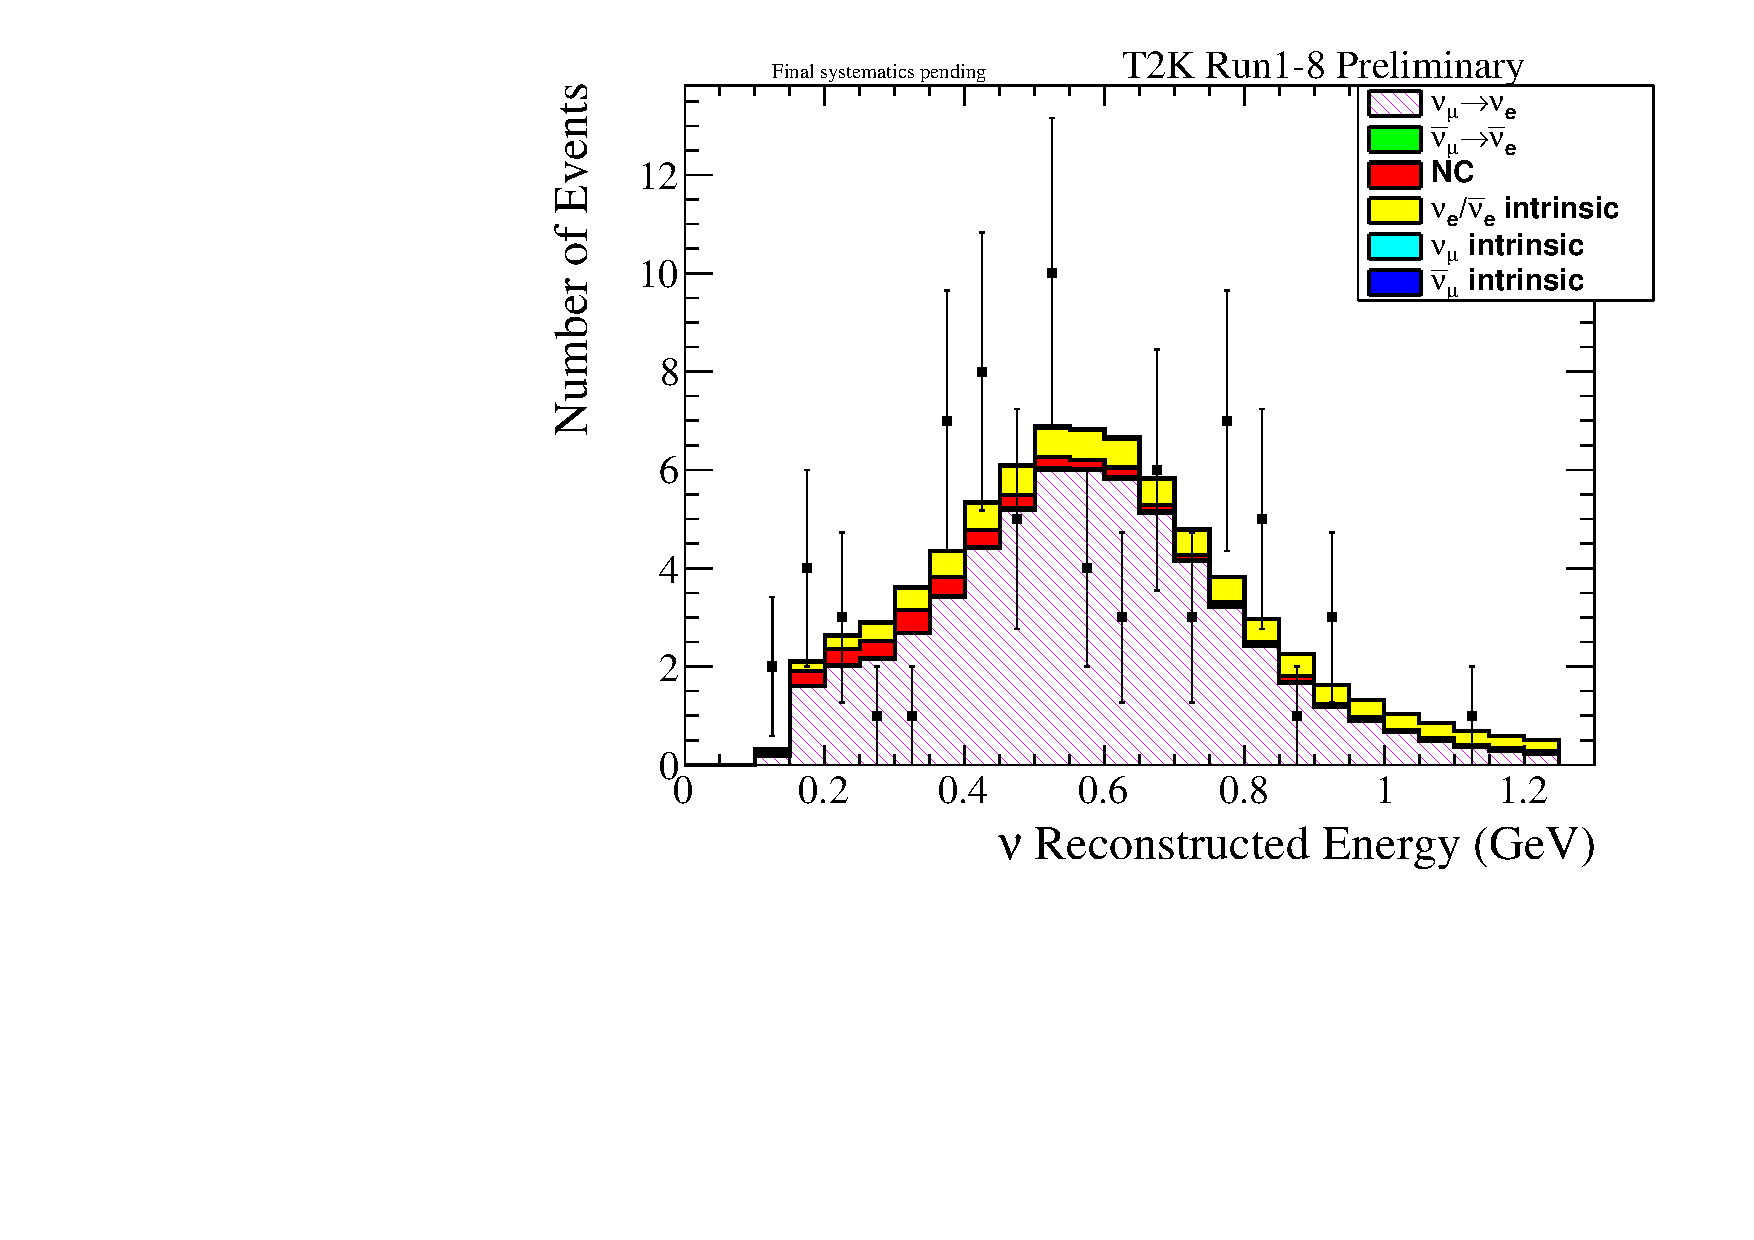
\includegraphics[width=0.9\textwidth]{spectra/erec_spectrum_osc_asimovpf_1Re_data}
		\caption{Electron-like, neutrino mode}
	\end{subfigure}
	\begin{subfigure}[b]{0.49\textwidth}
		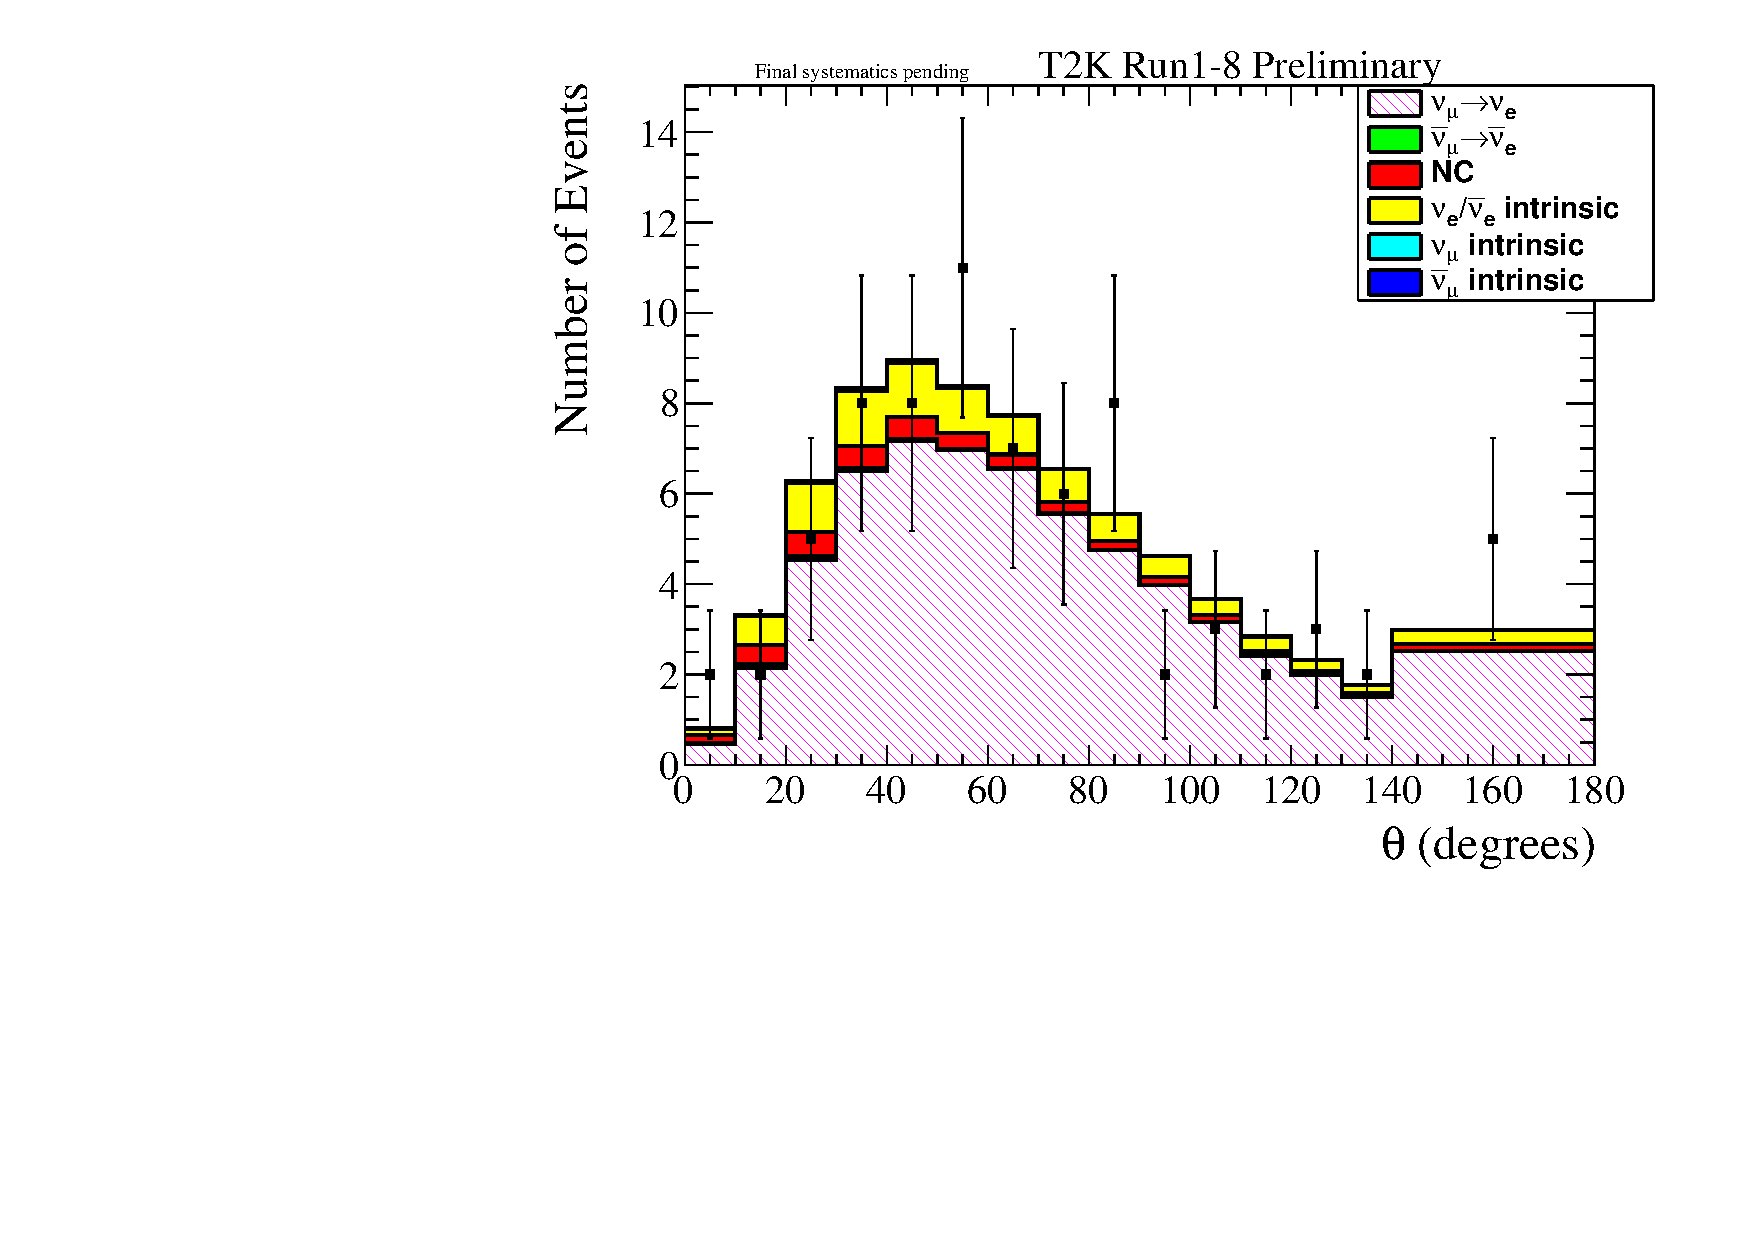
\includegraphics[width=0.9\textwidth]{spectra/theta_spectrum_osc_asimovpf_1Re_data}
		\caption{Electron-like, neutrino mode}
	\end{subfigure}

	\begin{subfigure}[b]{0.49\textwidth}
		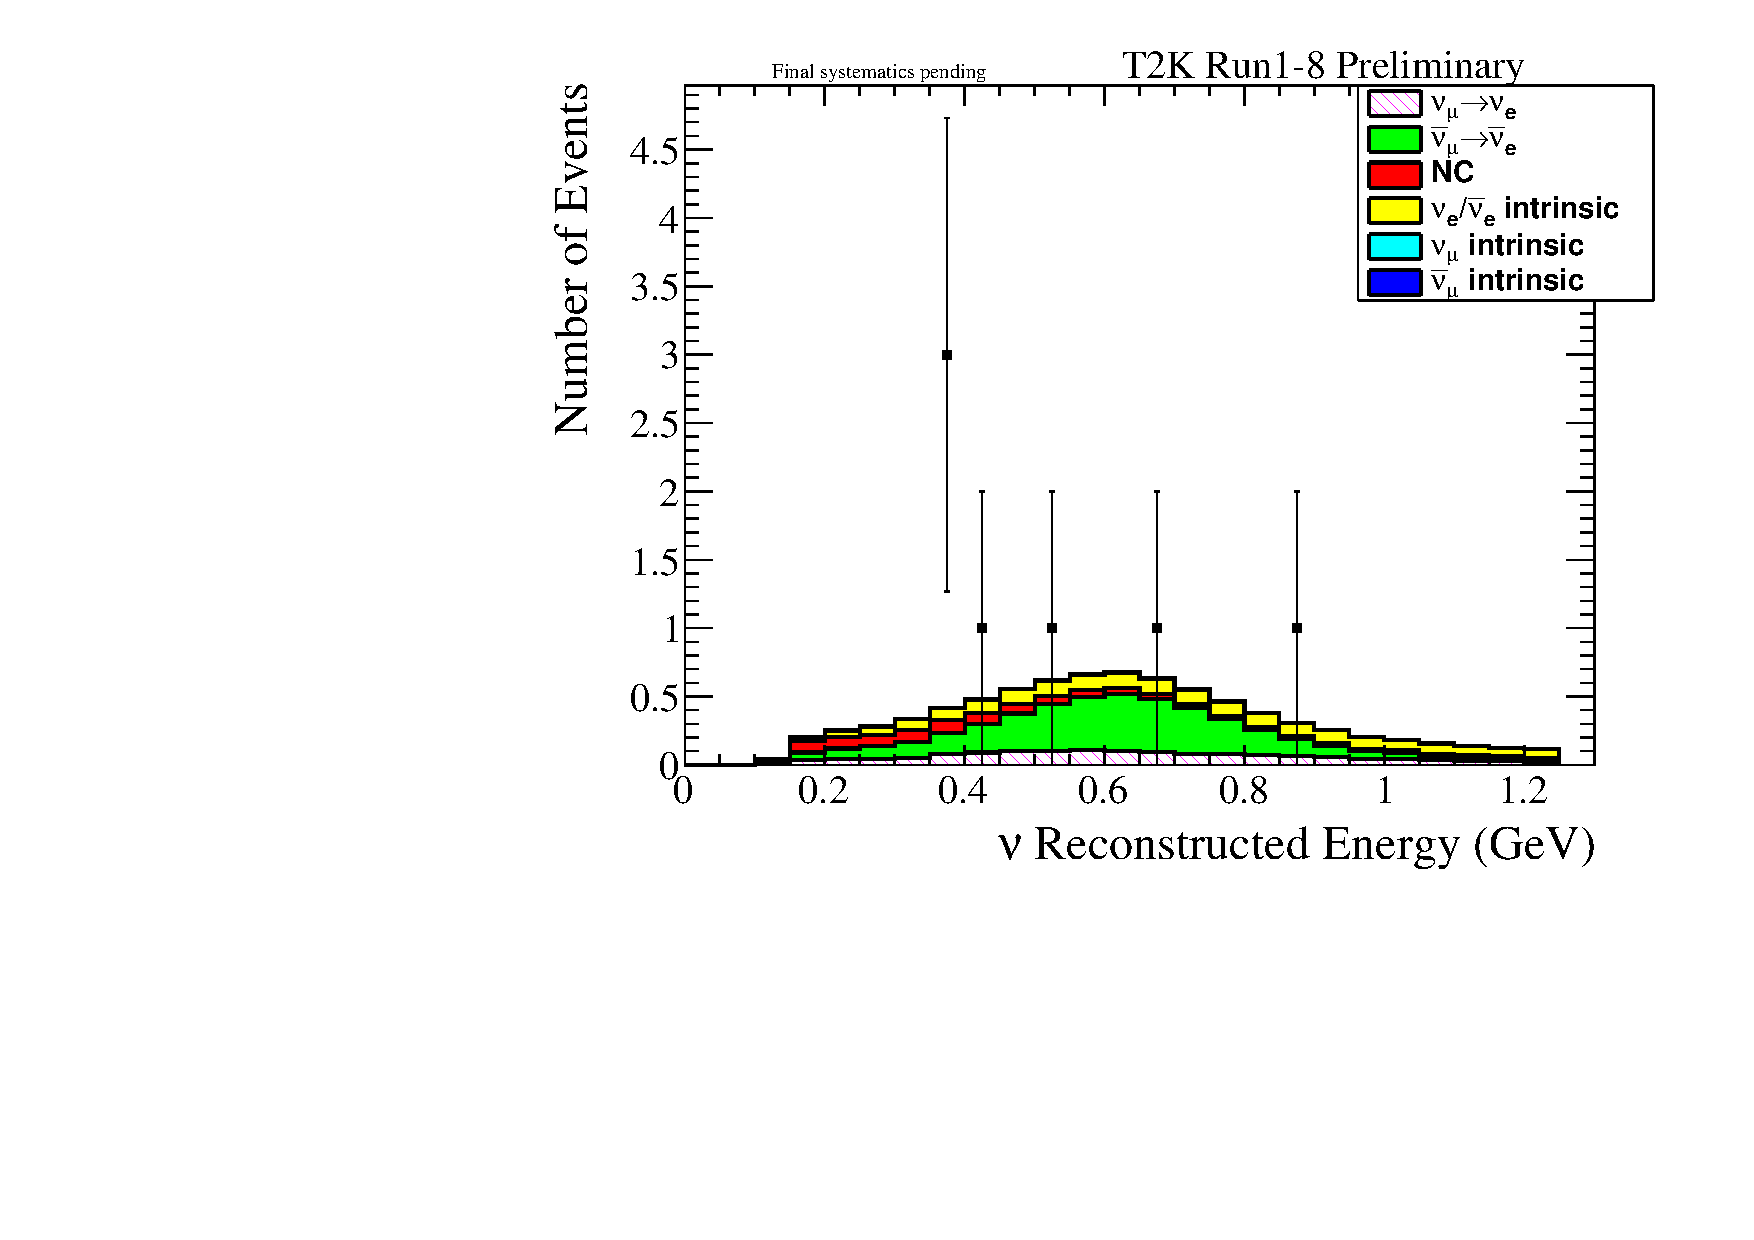
\includegraphics[width=0.9\textwidth]{spectra/erec_spectrum_osc_asimovpf_RHC1Re_data}
		\caption{Electron-like antineutrino mode}
	\end{subfigure}
	\begin{subfigure}[b]{0.49\textwidth}
		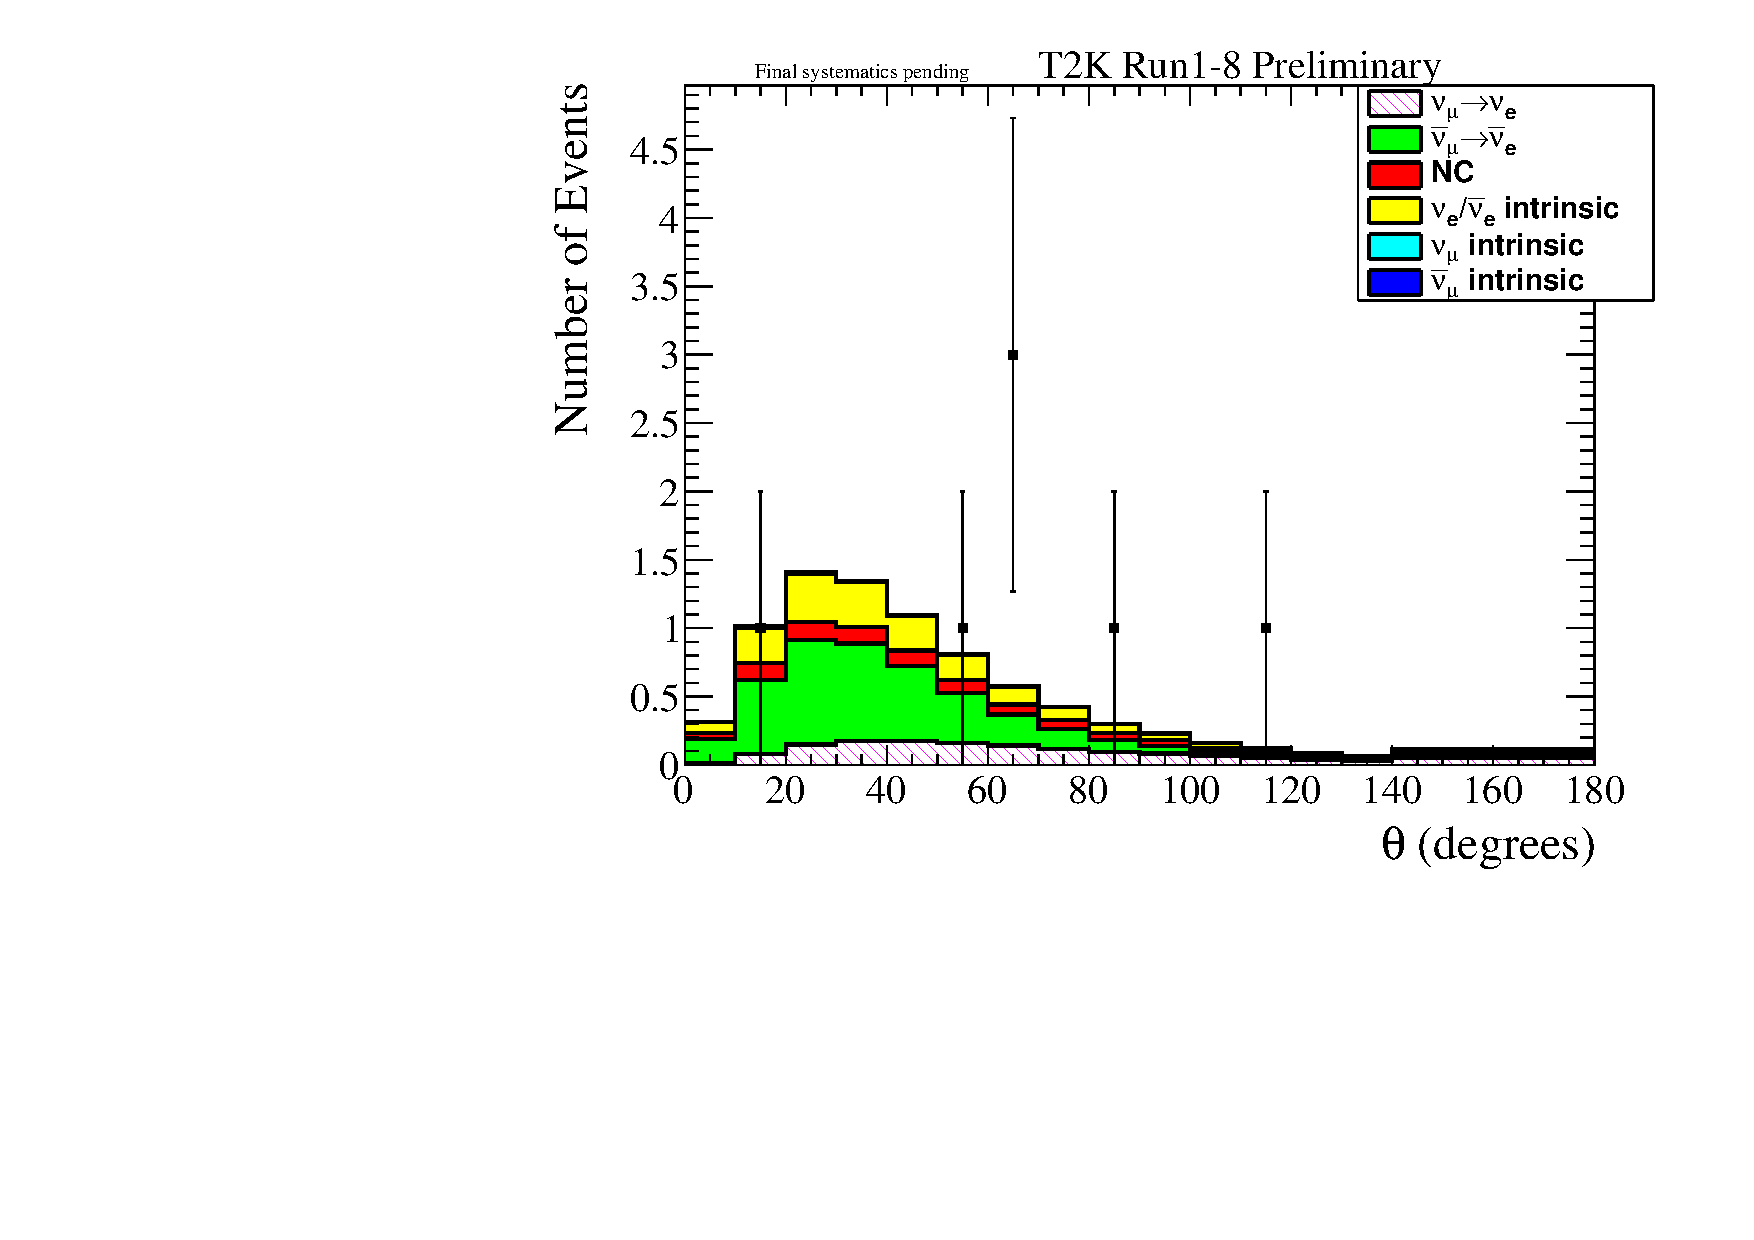
\includegraphics[width=0.9\textwidth]{spectra/theta_spectrum_osc_asimovpf_RHC1Re_data}
		\caption{Electron-like antineutrino mode}
	\end{subfigure}

	\begin{subfigure}[b]{0.49\textwidth}
		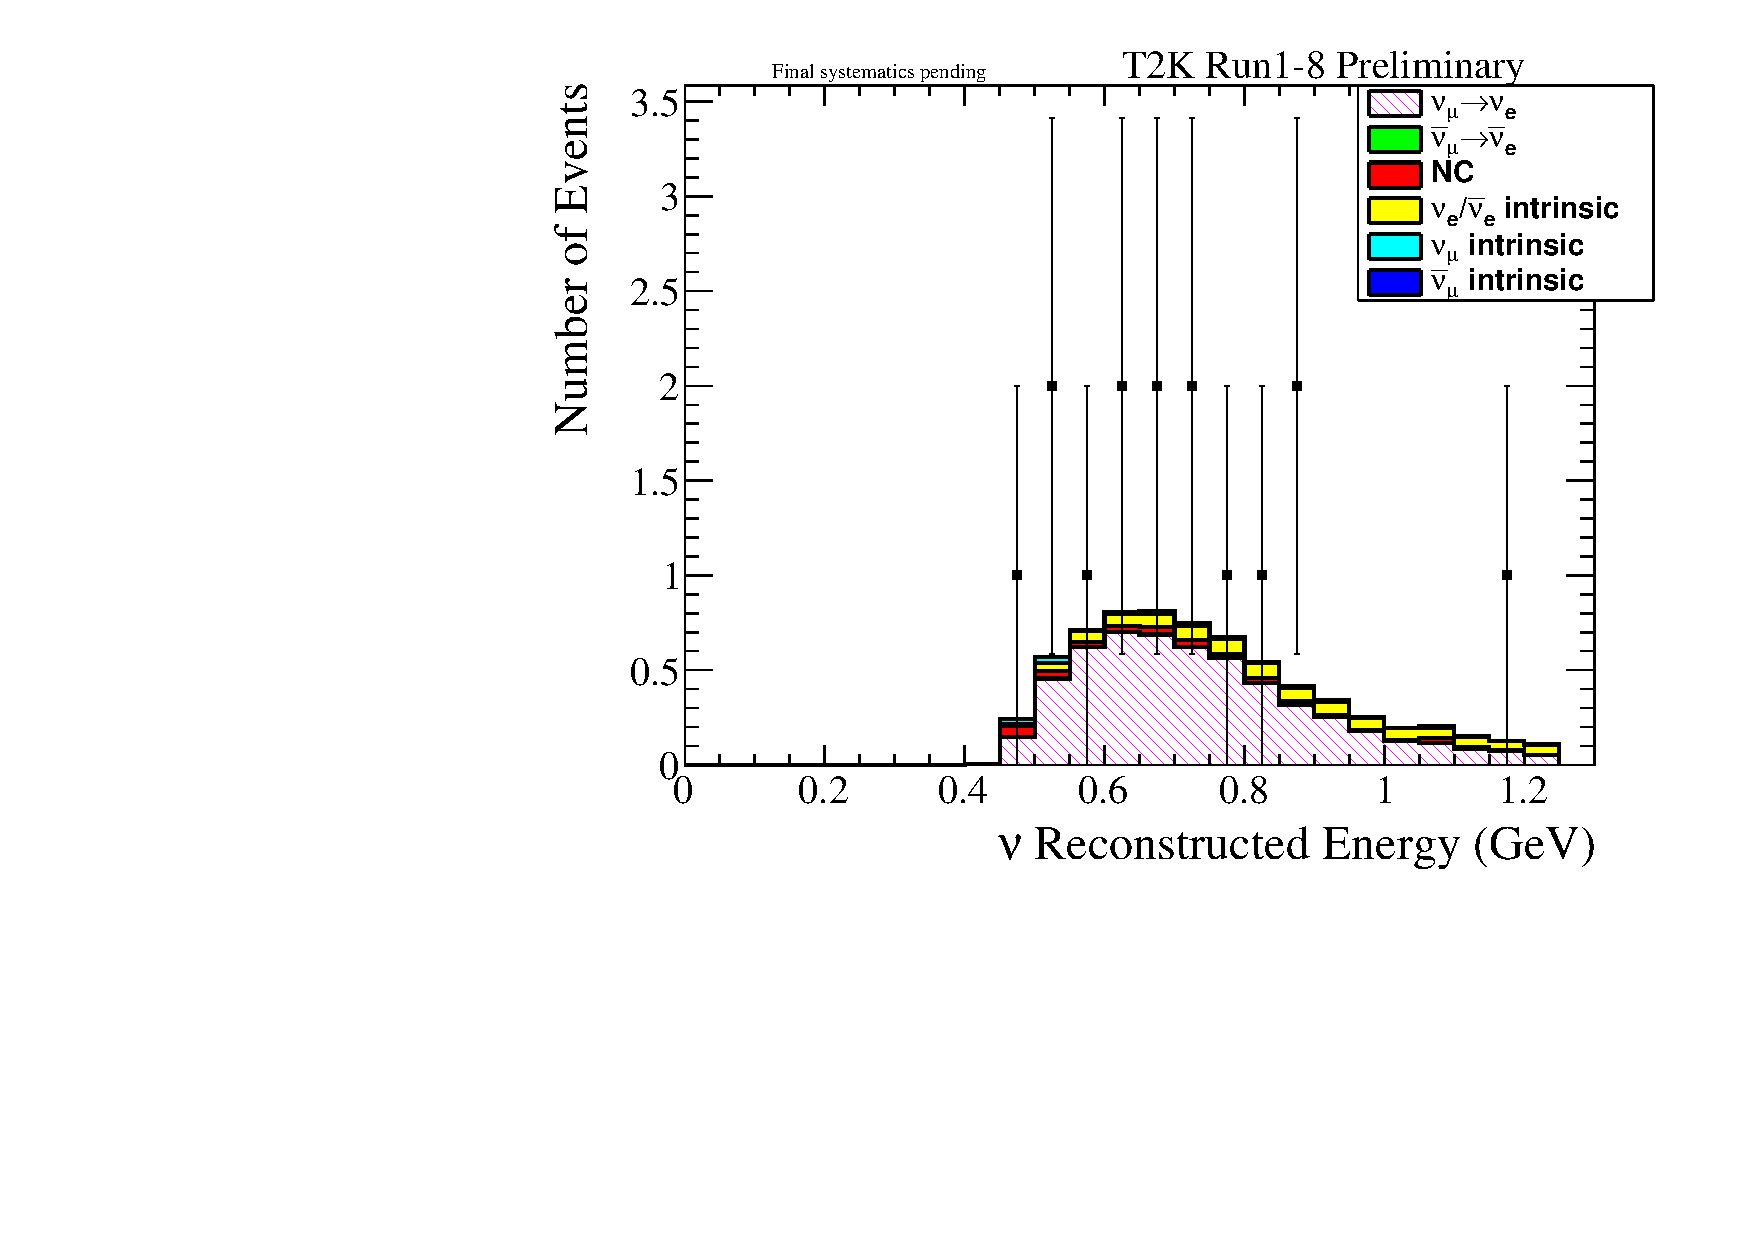
\includegraphics[width=0.9\textwidth]{spectra/erec_spectrum_osc_asimovpf_MultiRe_data}
		\caption{\nueCConepi-like, neutrino mode}
	\end{subfigure}
	\begin{subfigure}[b]{0.49\textwidth}
		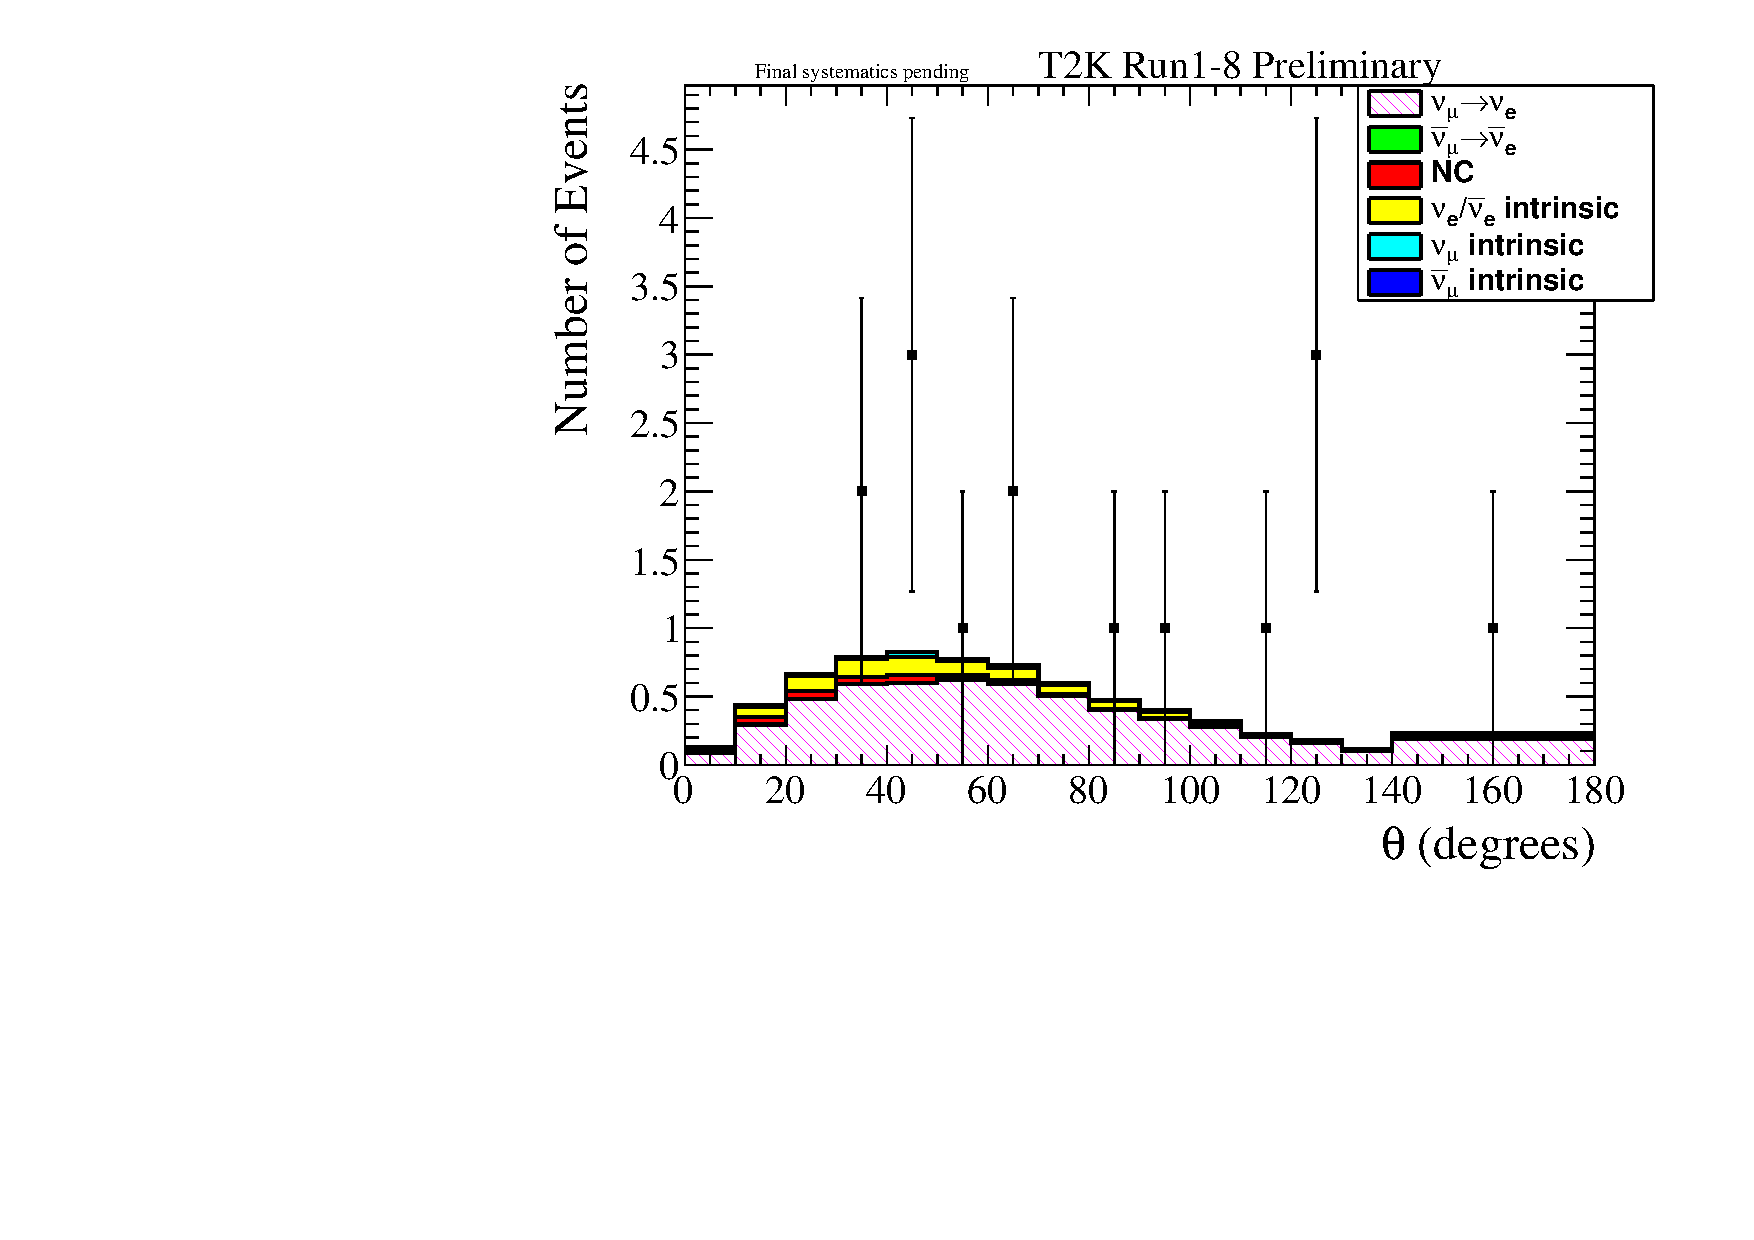
\includegraphics[width=0.9\textwidth]{spectra/theta_spectrum_osc_asimovpf_MultiRe_data}
		\caption{\nueCConepi-like, neutrino mode}
	\end{subfigure}
	\caption {
		Predicted spectra and observed events (points). The $e$-like, including \nueCConepi, distributions are functions of both the reconstructed neutrino energy and the reconstructed angle between the outgoing lepton and the neutrino direction, with the projections in each variable shown here. The distributions correspond to the statistics collected in the full \RunPeriod data set. The spectra are generated with the systematic parameters described in \cref{sec:systematics} and the oscillation parameters corresponding to the best-fit values from the data fit (solar parameters at PDG 2016).
	}
	\label{fig:asimovpf_spectra_mc_data_elike_1D}
\end{figure*}
\clearpage